\documentclass[12pt, a4paper,usenames,dvipsnames]{article}
\usepackage[utf8]{inputenc}
\usepackage[english]{babel}
\usepackage{amsmath,amssymb,amsthm} 
\usepackage{graphicx}
\usepackage{siunitx}
    \sisetup{exponent-product = \cdot} 
    \sisetup{separate-uncertainty = true}
\usepackage[margin=20mm, tmargin=30mm,headheight=15pt ]{geometry}
\usepackage[table]{xcolor}
\usepackage{fancyhdr}
\usepackage{framed}
\usepackage{caption}
\usepackage{subcaption}
\usepackage{lastpage}  
\pagestyle{fancy}
    \fancyhf{}
    \rhead{Project 3}
    \lhead{MA2501}
    \rfoot{Page \thepage \ of \pageref{LastPage}}
\fancypagestyle{noheader}{
  \fancyhf{}% Clear header/footer
  \renewcommand{\headrulewidth}{0pt}% No header rule
  \rfoot{Page \thepage \ of \pageref{LastPage}}
}
\usepackage{tikz}
\usetikzlibrary{calc}
\usetikzlibrary{patterns}
\usetikzlibrary{positioning}
\usepackage{lettrine}
\title{Project 3 - MA2501}
\author{Anna Bakkebø\And Thomas Schjem \And Endre Sørmo Rundsveen}
\usepackage{sectsty}
\usepackage{bm}



\definecolor{XKCDpale}{RGB}{255,249,208}
\definecolor{XKCDcrimson}{RGB}{140,0,15}
\definecolor{XKCDpalegray}{RGB}{253,253,254}
\definecolor{tableBack}{RGB}{246, 246, 240}


\sectionfont{\color{XKCDcrimson}}
\subsectionfont{\color{XKCDcrimson}}
\usepackage{listings}%Code show
\lstdefinestyle{mystyle}{
    backgroundcolor=\color{XKCDpalegray},
    commentstyle=\color{YellowGreen},
    keywordstyle=\color{XKCDcrimson}\bfseries,
    numberstyle=\tiny,
    stringstyle=\color{OliveGreen},
    basicstyle=\footnotesize,
    breakatwhitespace=false,         
    breaklines=true,                 
    captionpos=t,                    
    keepspaces=true,                 
    numbers=left,                    
    numbersep=1pt,                  
    showspaces=false,                
    showstringspaces=false,
    showtabs=false,                  
    tabsize=1,
    xleftmargin=0.5em,
    frame=topline
}
 
\lstset{style=mystyle}
\renewcommand\vec{\mathbf}

\begin{document}

\begin{titlepage}
    \newgeometry{margin=20mm,tmargin=110mm}
    \begin{tikzpicture}[remember picture,overlay]
        \fill[color=XKCDpale] ($(current page.south west)+(0cm,15cm)$) rectangle (current page.north east);
        \foreach \x in {2,3,4,5,6,7,8}
            {\fill[tableBack] (\x cm, 1)--(\x cm, {3+1.15*sin(0.5*pi*\x r)*exp(-\x/4)})--(\x +1,{3+1.15*sin(0.5*pi*(\x+1) r)*exp(-(\x+1)/4)})--(\x +1,1) --cycle;
            \draw[dashed] (\x cm, {3+1.15*sin(0.5*pi*\x r)*exp(-\x/4)})--(\x +1,{3+1.15*sin(0.5*pi*(\x+1) r)*exp(-(\x+1)/4)});}
        \draw[thick,->] (-2,1)--(15,1);
        \draw[thick,->] (-2,1)--(-2,8);
        \foreach \x in {2,3,4,5,6,7,8,9}
            {\draw (\x cm,1cm+2pt)--+(0,-4pt);
            \draw[dashed] (\x ,1)--(\x,{3+1.15*sin(0.5*pi*\x r)*exp(-\x/4)});}
        \node[anchor=north] at (2,1){\(a\)};
        \node[anchor=north] at(9,1){\(b\)};
        \draw[Mahogany, thick, domain=2:9] plot[samples=100] (\x, {3+1.15*sin(0.5*pi*\x r)*exp(-\x/4)});
        
    \end{tikzpicture}
  
    {\noindent \Huge \color{Brown}{\underline{Project 3 - MA2501}}}\\
    
    {\noindent\large \color{Brown}{Anna Bakkebø\\Thomas Schjem\\Endre Sørmo Rundsveen}}\\
    \raggedright
    \hfill \break
    \lettrine[lraise=0.15]{T}{} his document is the report for our third project in Numerical Methods - MA2501 the spring semester of 2019. The project mainly focuses on numerical integrations techniques and are based on the Newton-Cotes quadrature formula. First we familiarize ourself with the adaptive simpson method, before we continue with the Romber method, and lastly we end by exploring both the Runge-Kutta implicit integration method and the improved Euler method. \\ 
    \hspace{10pt}Note that we use some place to talk about the theory behind the methods. This is mainly for our own benefit so we can easily consult this document at a later time to repeat. For readers well-versed in the underlying theory, these sections can be quite unnecessary, and can thus be skipped. 
    % \begin{lstlisting}[language=Python]
    % import matplotlib
    % import matplotlib.pyplot as plt
    % import numpy as np
    % import sumpy as symp\end{lstlisting}
\end{titlepage}
\restoregeometry


\section*{Problem 1}
\subsection*{a)}
\subsubsection*{Theory}
The composite Simpson method for integrating a function 
\[\int_a^bf(x)dx\] 
divide the interval \([a,b]\) in \(n\) subintervals\\ \([x_{i-1},x_i]\), \(i=1,\cdots,n\), which it runs the Simpson method on, where \((x_i)_{i=0}^{i=n}\) is equidistant nodes \[a=x_0<x_1<\cdots<x_{n-1}<x_n=b\]

This will generally give a better approximation than to only run the Simpson method over the original interval, but it happens that a finer partition of an interval doesn't result in better approximation, e.g. if the function is a polynomial of grade 3 or lower the Simpson method will give the exact solution. In these situations, it is superfluous too further divide the interval and thus do more calculations. One would therefore prefer if the method could decide on whether it has reached a sufficient fine partition or not.

This motivates the Adaptive Simpson Method (ASM). We take a general subinterval \([a_j,b_j]\) and use Simpson to get an estimate \(I_0=S(a_j,b_j)\) and then use the composite Simpson method on it with two subintervals to get the estimate \(I_1\). If \(I_0\) and \(I_1\) is sufficiently close, we can conclude that \(I_0\) is reasonably close, so any further division of the subinterval will be superfluous. Otherwise the subinterval is divided into two smaller subintervals on which the same procedure is used. This gives a recursive formula. 

To give a criteria for when \(I_0\) and \(I_1\) is sufficiently close, we look at the relationship between the error bound for Simpson on one interval and composite Simpson with two subintervals. The absolute error for the Simpson method over \([a_j,b_j]\) (\(\varepsilon_{[a_j,b_j]}\)) is bounded by 
\[\varepsilon_{[a_j,b_j]}\leq \frac{(b_j-a_j)^5}{2880}M_4,\quad M_4=\max_{\eta\in(a_j,b_j)}|f^{(4)}(\eta)|\]
If we use the simpson method on the two subintervals \([a_j,c_j],[c_j,b_j]\) where \(c_j=\frac{a_j+b_j}{2}\), we can see that the sum of the two errors is bounded by 
\begin{equation*}
    \begin{split}
        \varepsilon_{[a_j,c_j]}+\varepsilon_{[c_j,b_j]}\leq& \frac{(c_j-a_j)^5}{2880}M_4+\frac{(b_j-c_j)^5}{2880}M_4\\
        =&2\cdot\left(\frac{b_j-a_j}{2}\right)^5\cdot\frac{M_4}{2880}\\
        =&\frac{1}{16}\cdot\frac{(b_j-a_j)^5}{2880}M_4
    \end{split}
\end{equation*}
where \(M_4=\max_{\eta \in (a_j,b_j)}|f^{(4)}(\eta)|\). Hence the difference in error for the composite Simpson method with two subintervals on \([a_j,b_j]\) and Simpson method on the same interval is
\begin{equation*}
    \begin{split}
        \varepsilon_{[a_j,b_j]}-\varepsilon_{[a_j,c_j]}-\varepsilon_{[c_j,b_j]}\approx \frac{15}{16}\cdot\frac{(b_j-a_j)^5}{2880}M_4
    \end{split}
\end{equation*}
Using 
\[\int_a^bf(x)dx\approx S(a,b)+\varepsilon_{[a,b]}\]
we can rewrite this as
\[\frac{16}{15}\left(S(a_j,b_j)-S(a_j,c_j)-S(c_j,b_j)\right)\approx\frac{(b_j-a_j)^5}{2880}M_4\]
This result in
\begin{equation*}
    \begin{split}
        \int_{a_j}^{b_j}f(x)dx-I_1\approx&\frac{1}{16}\cdot\frac{(b_j-a_j)^5}{2880}M_4\\
         \approx&\frac{1}{15}\left(S(a_j,b_j)-S(a_j,c_j)-S(c_j,b_j)\right)\\
         =&\frac{1}{15}(I_0-I_1)
    \end{split}
\end{equation*}
Finally
\[\left|\int_{a_j}^{b_j}f(x)dx-I_1\right|\approx\frac{1}{15}\left|I_0-I_1\right|\]
Thus, if \(\frac{1}{15}|I_0-I_1|<TOL\), \(I_1\) is within the tolerance limit set, over that subinterval. Therefore we can use this as en estimate of whether \(I_0\) and \(I_1\) is sufficiently close. For each time we divide a subinterval into two smallet subintervals, we half the tolerance for the method on those intervals.  


\thispagestyle{noheader}
\newgeometry{margin=20mm, tmargin=0.55\paperwidth,headheight=15pt}
\refstepcounter{figure}
\label{fig:graph}
\begin{tikzpicture}[remember picture,overlay]
    \fill[color=XKCDpale] ($(current page.north west)-(0,{0.6\paperwidth})$) rectangle (current page.north east);
    \node (graph) at ($(current page.north)-(0,0.3\paperwidth)$) {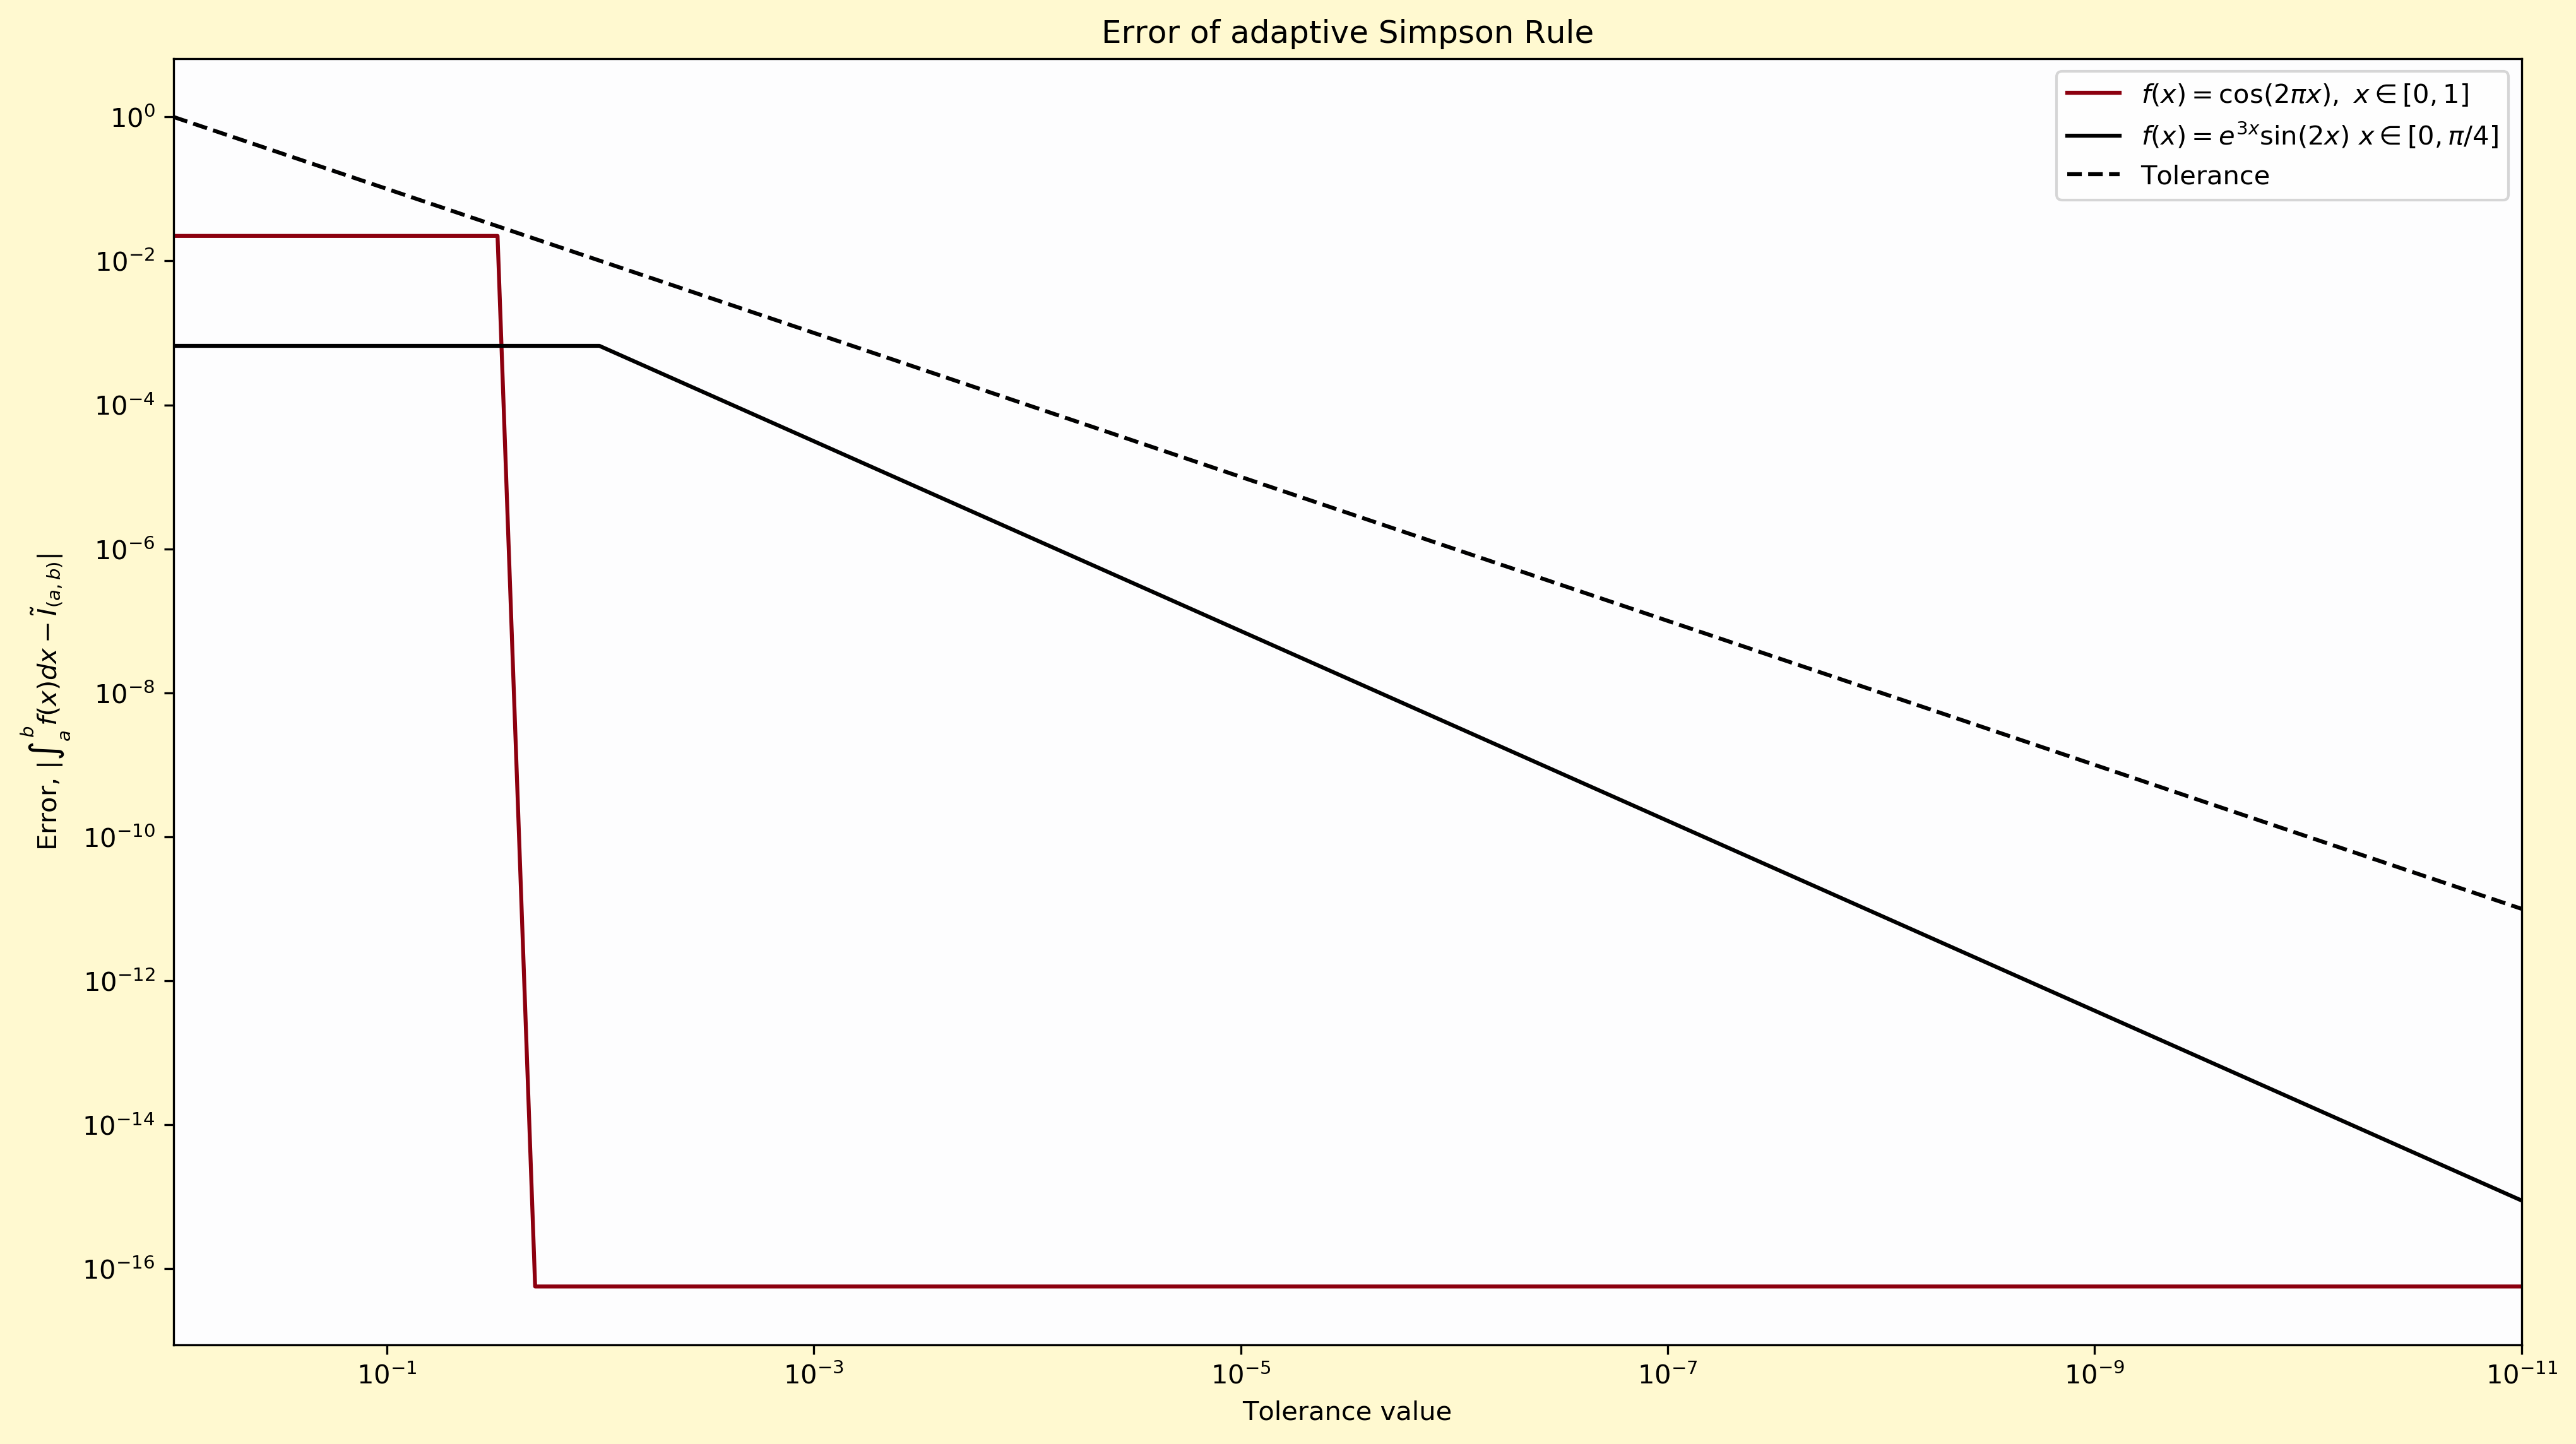
\includegraphics[width=0.9\paperwidth]{pltAdpSimp.png}};
    \node[below= 0.15cm  of graph] {Figure \arabic{figure}: The errors of the adaptive Simpson Rule with decreasing tolerance, for different functions.};
\end{tikzpicture}

\subsection*{b)}
We have integrated a test function which checks that the errors for the given functions are below the set error bound. Also from Figure \ref{fig:graph}, one can observe that the adaptive Simpson method gives a result with a error below the tolerance for tolerance values in the range \([10,10^{-10}]\). Further it would seem as the cosine function is especially good approximated after a tolerance of about \(10^{-1.8}\). In table \ref{tab:simps} the values from a tolerance of \(10^{-7}\) is reproduced, and these are consistent with the afforementioned graph.
\begin{table}[h]
\centering
\begin{tabular}{p{2cm}p{2.5cm}ll}

\rowcolor{XKCDpale}$\textbf{f(x)}$                     & \textbf{Exact}               & \textbf{Simpson} & \textbf{Error} \\ \rowcolor{tableBack}
$cos(2 \pi x)$, \newline$x \in [0, 1]$      & 0                            & 0          & 0       \\ \rowcolor{tableBack}
$e^{3x}sin(2x)$, \newline$x \in [0, \dfrac{\pi}{4}]$ & $\frac{1}{13}(2+3e^{3\pi/4})$ \newline$\approx 2.588629$& 2.588629          & 6.3489e-10       \\ 
\end{tabular}
\caption{Values from the Simpson method ran on the respective functions ($f(x)$), with tolerance $1\cdot10^{-7}$, and rounded up after the 14 decimal.}
\label{tab:simps}
\end{table}
\restoregeometry
\subsection*{c)}
\subsubsection*{Theory}
The composite Trapezium rule follows the same idea as the composite Simpson method. Here we are to explore another method which actively adapts itself until it reaches a good result, in an effort to minimize needless work. The main difference from ASM is that this method is more global. ASM tried to exploit that Simpson can work great at some local neighbourhoods in the given interval, but Romberg method, which we shall soon familiarize, uses more global properties over the whole interval.

First, lets look at the error of the composite 

\thispagestyle{noheader}
\newgeometry{margin=20mm, tmargin=0.55\paperwidth,headheight=15pt}
\refstepcounter{figure}
\label{fig:graph}
\begin{tikzpicture}[remember picture,overlay]
    \fill[color=XKCDpale] ($(current page.north west)-(0,{0.6\paperwidth})$) rectangle (current page.north east);
    \node (graph) at ($(current page.north)-(0,0.3\paperwidth)$) {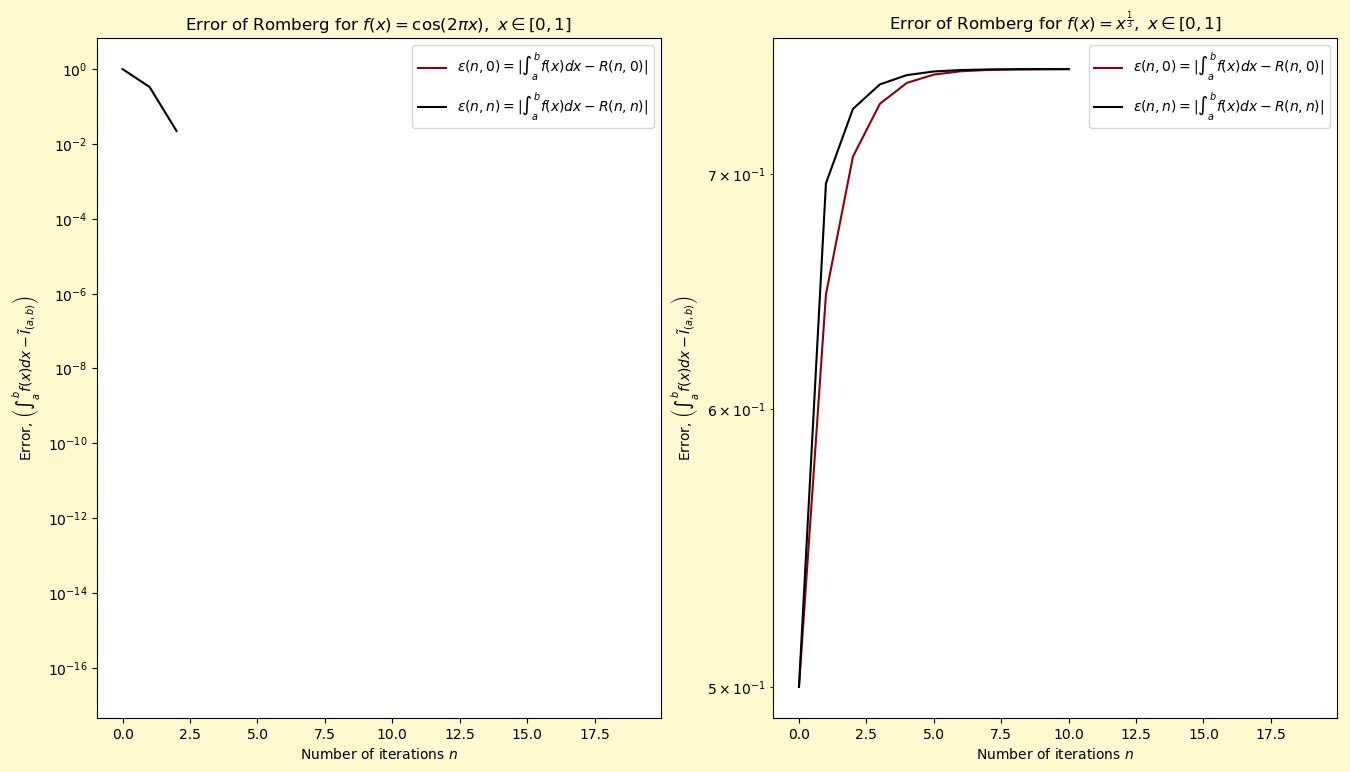
\includegraphics[width=0.9\paperwidth]{pltRombConv.png}};
    \node[below= 0.15cm  of graph] {Figure \arabic{figure}: The errors of the adaptive Simpson Rule with decreasing tolerance, for different functions.};
\end{tikzpicture}
\subsection*{d)}
\restoregeometry
\end{document}
